% ------------------------------------------------------------------------------
% TYPO3 CMS 6.2 LTS - What's New - Chapter "Responsive Images" (English Version)
%
% @author	Michael Schams <schams.net>
% @license	Creative Commons BY-NC-SA 3.0
% @link		http://typo3.org/download/release-notes/whats-new/
% @language	English
% ------------------------------------------------------------------------------
% Chapter: Responsive Images
% ------------------------------------------------------------------------------
\section{Responsywne Obrazki}
\begin{frame}[fragile]
	\frametitle{Responsywne Obrazki}

	\begin{center}\huge{Rozdział 2:}\end{center}
	\begin{center}\huge{\color{typo3darkgrey}\textbf{Responsywne Obrazki}}\end{center}

\end{frame}

% ------------------------------------------------------------------------------
% Select Screen Size In Page Preview
% ------------------------------------------------------------------------------

\begin{frame}[fragile]
	\frametitle{Responsywne Obrazki}
	\framesubtitle{Wybierz Wielkość Ekranu W Podglądzie Strony}

	\begin{itemize}
		\item W edytorze w module "View" możemy wybrać różne rozmiary ekranu, aby testować responsywne strony 
	\end{itemize}

	\begin{figure}
		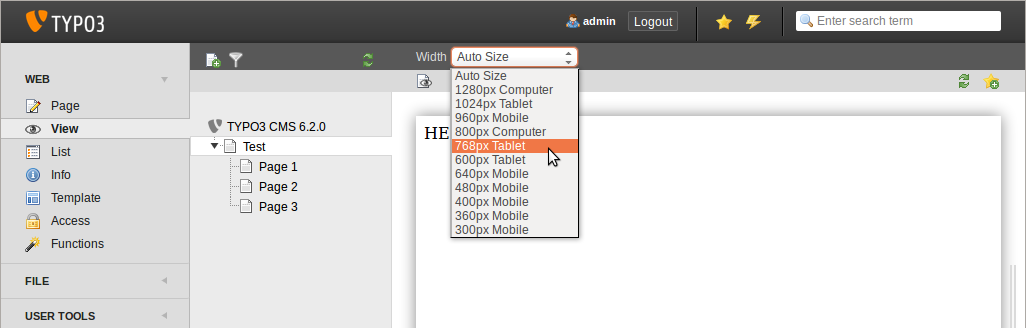
\includegraphics[width=0.95\linewidth]{Images/ResponsiveImages/ScreenSizeInPagePreview.png}
	\end{figure}

\end{frame}

% ------------------------------------------------------------------------------
% Customize Available Screen Sizes
% ------------------------------------------------------------------------------

\begin{frame}[fragile]
	\frametitle{Responsywne Obrazki}
	\framesubtitle{Dostępne Niestandardowe Rozmiary Ekranu}

	\begin{itemize}
		\item Rozmiary Ekranu są konfigurowalne przez "PageTSconfig":

		\lstset{
			basicstyle=\fontsize{7}{9}\selectfont\ttfamily
		}

		\begin{lstlisting}
			mod.web_view.previewFrameWidths {
			  1780.label = <any LLL or string>
			  1780.height = 145
			}
		\end{lstlisting}

		\item Szerokość jest definiowana przez klucz (tutaj: 1780), podanie wysokości nie jest obowiązkowe
		\item Domyślne rozmiary można znaleźć w pliku:\newline
			\small\texttt{typo3/sysext/core/Configuration/DefaultConfiguration.php}\normalsize
		\item Etykiety mogą być zdefiniowane przez "PageTSconfig":

		\begin{lstlisting}
			mod.web_view.previewFrameWidths {
			  1280.label = LLL:EXT:viewpage/Resources/Private/Language/locallang.xlf:computer
			  1024.label = LLL:EXT:viewpage/Resources/Private/Language/locallang.xlf:tablet
			}
		\end{lstlisting}

	\end{itemize}

\end{frame}

% ------------------------------------------------------------------------------
% Responsive Image Galleries
% ------------------------------------------------------------------------------

\begin{frame}[fragile]
	\frametitle{Responsywne Obrazki}
	\framesubtitle{Responsywne Galerie Obrazków}

	\begin{itemize}
		\item Dodane atrybuty do implementacji responsywnych galerii obrazków
		\item Rozszerzony "CSS styled content" na potrzeby responsywnych galerii obrazków
		\item Przykład: HTML5 (wymaga \texttt{config.doctype = html5})\newline

			TYPO3 CMS < 6.2:

			\lstset{
				basicstyle=\fontsize{7}{9}\selectfont\ttfamily
			}

			\begin{lstlisting}
				<div class="csc-textpic-imagewrap">...</div>
			\end{lstlisting}

			TYPO3 CMS >= 6.2:

			\begin{lstlisting}
				<div class="csc-textpic-imagewrap"
				  data-csc-images="{register:imageCount}"
				  data-csc-cols="{field:imagecols}">...</div>
			\end{lstlisting}

	\end{itemize}

\end{frame}

% ------------------------------------------------------------------------------
% Responsive Image Rendering
% ------------------------------------------------------------------------------

\begin{frame}[fragile]
	\frametitle{Responsywne Obrazki}
	\framesubtitle{Responsywne Renderowanie Obrazków}

	\begin{itemize}
		\item Obrazy cObject renderuje tzw. "sourceCollection" do wspierania różnych rozdzielczości ekranu
		\item Responsywne renderowanie obrazu dla cObjects "text/image" i "image" wymaga dwóch ustawień w stałym Edytorze:

			\texttt{styles.content.imgtext.responsive}\newline
			\texttt{styles.content.imgtext.layoutKey}

		\item Opcje:

			\begin{itemize}
				\item \texttt{default}:	\tabto{2cm} domyślnie \texttt{<img>}-tag
				\item \texttt{srcset}:	\tabto{2cm} \texttt{<img>}-tag z alternatywnymi źródłami takimi jak srcset-attribute
				\item \texttt{picture}:	\tabto{2cm} \texttt{<picture>}-tag z source-child-tags
				\item \texttt{data}:	\tabto{2cm} \texttt{<img>}-tag z alternatywnymi źródłami jak data-attributes
			\end{itemize}

	\end{itemize}

\end{frame} 

% ------------------------------------------------------------------------------
% Property: layoutKey
% ------------------------------------------------------------------------------

\begin{frame}[fragile]
	\frametitle{Responsywne Obrazki}
	\framesubtitle{Właściwość: layoutKey}

	\begin{itemize}
		\item \texttt{layoutKey} definiuje renderowany wygląd\newline
			(jest to kod HTML, używany przy tagu \texttt{<img>})
		\item Każda opcja pokazuje unikalne zachowania przy renderowaniu HTML-a
		\item Opcja \texttt{default} renderuje \texttt{tag <img>} tradycyjnie\newline
			(powinna być użyta, jeśli frontend nie jest responsywny)
		\item Wdrożenie responsywnego wyglądu wymaga różnych rozmiarów obrazków przy różnych rozdzielczościach i rozmiarach ekranu
		\item W zależności od HTML-a, możliwości przeglądarki i JavaScript-u:

			\begin{itemize}
				\item użycie jednego z domyślnych wyglądów lub
				\item zdefiniowanie własnego
			\end{itemize}

	\end{itemize}

\end{frame}

% ------------------------------------------------------------------------------
% Property: layout
% ------------------------------------------------------------------------------

\begin{frame}[fragile]
	\frametitle{Responsywne Obrazki}
	\framesubtitle{Właściwość: layoutKey}

	\lstset{
		basicstyle=\tiny\ttfamily
	}

	\begin{lstlisting}
		layoutKey = {$styles.content.imgtext.layoutKey}
		layout {
		  default {
		    element = <img src="###SRC###" width="###WIDTH###" height="###HEIGHT###" ###PARAMS###
		      ###ALTPARAMS### ###BORDER######SELFCLOSINGTAGSLASH###>
		  }
		  srcset {
		    element = <img src="###SRC###" srcset="###SOURCECOLLECTION###" ###PARAMS###
		      ###ALTPARAMS### ###SELFCLOSINGTAGSLASH###>
		    source = |*|###SRC### ###SRCSETCANDIDATE###,|*|###SRC### ###SRCSETCANDIDATE###
		  }
		  picture {
		    element = <picture>###SOURCECOLLECTION###<img src="###SRC###" ###PARAMS###
		      ###ALTPARAMS######SELFCLOSINGTAGSLASH###></picture>
		    source = <source src="###SRC###" media="###MEDIAQUERY###"###SELFCLOSINGTAGSLASH###>
		  }
		  data {
		    element = <img src="###SRC###" ###SOURCECOLLECTION### ###PARAMS###
		      ###ALTPARAMS######SELFCLOSINGTAGSLASH###>
		    source = data-###DATAKEY###="###SRC###"
		  }
		}
	\end{lstlisting}

\end{frame}

% ------------------------------------------------------------------------------
% Property: layout.[layoutKey].element
% ------------------------------------------------------------------------------

\begin{frame}[fragile]
	\frametitle{Responsywne Obrazki}
	\framesubtitle{Właściwość: layout.[layoutKey].element}

	\begin{itemize}
		\item \lstinline!###SRC###!\newline
			URL w atrybucie (patrz poniżej): \texttt{src}

		\item \lstinline!###WIDTH###!\newline
			Szerokość obrazka (w pikselach) dla atrybutu: \texttt{width}

		\item \lstinline!###HEIGHT###!\newline
			Wysokość obrazka (w pikselach) dla atrybutu: \texttt{height}

		\item \lstinline!###PARAMS###!\newline
			Dodatkowe parametry zdefiniowane w cObject IMAGE

		\item \lstinline!###ALTPARAMS###!\newline
		Dodatkowe alternatywne parametry zdefiniowane w cObject IMAGE
	\end{itemize}

\end{frame}

% ------------------------------------------------------------------------------
% Property: layout.[layoutKey].element
% ------------------------------------------------------------------------------

\begin{frame}[fragile]
	\frametitle{Responsywne Obrazki}
	\framesubtitle{Właściwość: layout.[layoutKey].element}

	\begin{itemize}
		\item \lstinline!###BORDER###!\newline
			Ramka (w pikselach) atrybutu: \texttt{border}

		\item \lstinline!###SELFCLOSINGTAGSLASH###!\newline
			Tag zamykający, przykład \texttt{<img ... />} vs. \texttt{<img ... >}\newline
			(zależy od \texttt{config.xhtmlDoctype} albo \texttt{config.doctype})

		\item \lstinline!###SOURCECOLLECTION###!\newline
			Opcjonalne obrazki, w zależności od używania responsywnego design-u.
			Dokładne wartości określa klucz: \texttt{layout.[layoutKey].source}
	\end{itemize}

\end{frame}

% ------------------------------------------------------------------------------
% Property: sourceCollection.[dataKey]
% ------------------------------------------------------------------------------

\begin{frame}[fragile]
	\frametitle{Responsywne Obrazki}
	\framesubtitle{Właściwość: sourceCollection.[dataKey]}

	\begin{itemize}
		\item Domyślnie sourceCollection z EXT:css\_styled\_content
		\item Rekomenduje się napisanie własnego "sourceCollection"

			\lstset{
				basicstyle=\tiny\ttfamily
			}

			\begin{lstlisting}
				sourceCollection {
				  small {
				    width = 200
				    srcsetCandidate = 600w
				    mediaQuery = (max-device-width: 600px)
				    dataKey = small
				  }
				  smallRetina {
				    if.directReturn = 1
				    width = 200
				    pixelDensity = 2
				    srcsetCandidate = 600w 2x
				    mediaQuery = (max-device-width: 600px) AND (min-resolution: 192dpi)
				    dataKey = smallRetina
				  }
				}
			\end{lstlisting}
	\end{itemize}

\end{frame}

% ------------------------------------------------------------------------------
% Further Resources (External Links)
% ------------------------------------------------------------------------------

\begin{frame}[fragile]
	\frametitle{Responsywne Obrazki}
	\framesubtitle{Przydatne linki}

	\begin{itemize}
		\item Przykłady działającego kodu:\newline
			\small\url{http://wiki.typo3.org/Responsive_Image_Rendering}\normalsize

		\item Artykuły Svena Wolfermanna na typo3.org:\newline
			\small\url{http://typo3.org/news/article/responsive-image-rendering-in-typo3-cms-62/}\normalsize

		\item Specyfikacja W3C:\newline
			\small\url{http://www.w3.org/html/wg/drafts/srcset/w3c-srcset/}\newline
			\small\url{http://www.w3.org/TR/html-picture-element/}

		\item Projekt grupy "Responsive Image Community Group":\newline
			\small\url{http://responsiveimages.org}\normalsize

	\end{itemize}

\end{frame}

% ------------------------------------------------------------------------------

